% This LaTeX was auto-generated from MATLAB code.
% To make changes, update the MATLAB code and export to LaTeX again.

\documentclass{article}

\usepackage[utf8]{inputenc}
\usepackage[T1]{fontenc}
\usepackage{lmodern}
\usepackage{graphicx}
\usepackage{color}
\usepackage{hyperref}
\usepackage{amsmath}
\usepackage{amsfonts}
\usepackage{epstopdf}
\usepackage[table]{xcolor}
\usepackage{matlab}

\sloppy
\epstopdfsetup{outdir=./}
\graphicspath{ {./cascade_1_images/} }

\begin{document}

\matlabtitle{Legged Mobility Assignment}


\vspace{1em}
\matlabheading{Part 1 Question 6}

\begin{matlabcode}
p_range = 0:0.04:0.25; % Distance to COP from ankle
v_0_range = 0:0.2:3; % Initial Velocity

[v_0,p] = meshgrid(v_0_range, p_range);

y_0 = 1 % height is fixed in LIPM model (here = 1 metre)
\end{matlabcode}
\begin{matlaboutput}
y_0 = 1
\end{matlaboutput}
\begin{matlabcode}

X_t = -p + sqrt(p.^2 + ((v_0.^2)*y_0)/9.81);

surf(p,v_0,X_t);
title('Capture Point plot')
ylabel('v_0')
xlabel('p')
zlabel('X_T')
\end{matlabcode}
\begin{center}
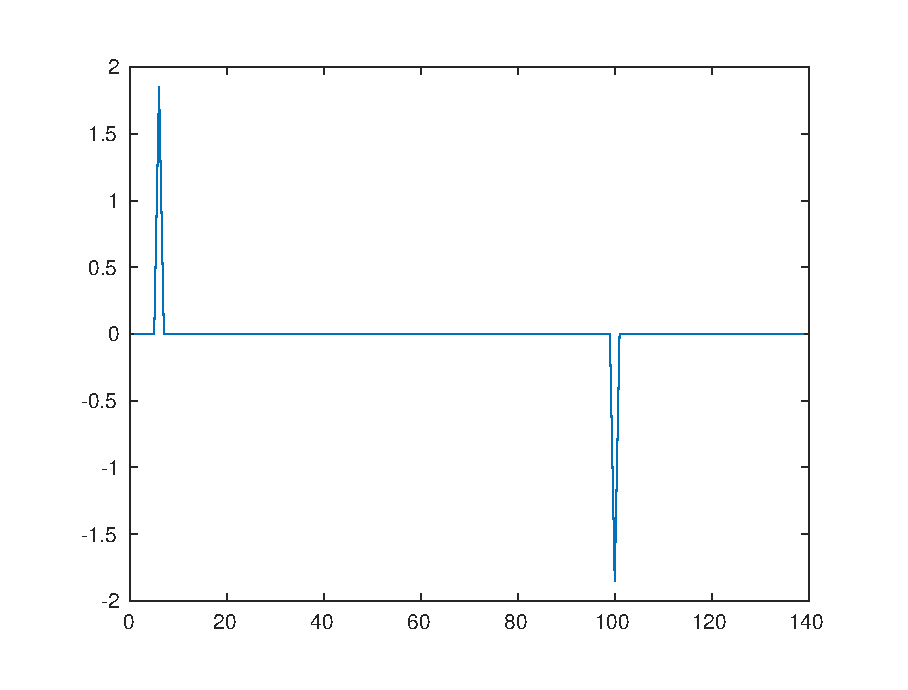
\includegraphics[width=\maxwidth{83.69292523833417em}]{figure_0.eps}
\end{center}

\vspace{1em}

\matlabheadingthree{Observations}

\begin{itemize}
\setlength{\itemsep}{-1ex}
   \item{\begin{flushleft} A velocity range of 0m/s - 3m/s was chosen as the average human walking speed was found to be 1.4m/s \end{flushleft}}
   \item{\begin{flushleft} The COP was varied from 0cm - 25cm to account for COP within the average human foot's polygon of support (assuming average human foot size = US 9 = 25cm). \end{flushleft}}
   \item{\begin{flushleft} When p=0, there is no torque available for the ankle to generate a balancing force, therefore the response would be to take a larger step ahead to compensate for this lack of ankle torque \end{flushleft}}
   \item{\begin{flushleft} As the COP moves further away from the ankle (but within the polygon of support), the available ankle torque increases and this can reduce the capture point distance as seen from the graph \end{flushleft}}
   \item{\begin{flushleft} As long as the COP (p) remains within the polygon of support and the capture point is small, ankle torque can be applied to balance the robot. However, even if COP is within the polygon of support but the X\_T value is large as in the below diagram where COP = 0.24m (within average human foot polygon) still has an X\_T = 0.74m \end{flushleft}}
\end{itemize}

\begin{par}
\begin{center}
\includegraphics[width=\maxwidth{54.99247365780231em}]{image_0}
\end{center}
\end{par}

\begin{itemize}
\setlength{\itemsep}{-1ex}
   \item{\begin{flushleft} this could mean that the velocity 3m/s is too high and the ankle torque required would be too high and infeasible for control. In such a situation, taking a step would almost be necessary. \end{flushleft}}
   \item{\begin{flushleft} Also, X\_T = 0.74 is approximately 3x the foot size for the average human which intuitively seems to be our usual capture point when walking. \end{flushleft}}
\end{itemize}


\vspace{1em}
\matlabheading{Part 2 Question 4 }

\matlabheading{Cascaded Controller}


\vspace{1em}
\begin{matlabcode}
% Define the system constants
r = 0.05; % radius of gear in metres
N = 41; % gear ratio
m = 80; % mass in Kgs
g = 9.81; % gravitational constant
J = 0.0005060; % motor inertia (rotor inertia) in Kgm2
k = 20000; % Nm (spring constant)

Kp_e1 = 8;
Kd_e1 = 1;

Kp_e2 = 10;
Kd_e2 = 1;

% Define the initial system parameters
y_des = 0.9;
F_s_des = 0;

thetha_des = 0;
 
y_0 = 1;
y = [1];
y_dot = 0;
y_ddot = 0;
 
thetha = 0;
thetha_dot = 0;
thetha_ddot = 0;
 
tau_m = [];

F_s_real = 0;
\end{matlabcode}


\vspace{1em}
\begin{par}
\begin{flushleft}
Define the controller
\end{flushleft}
\end{par}

\begin{matlabcode}
timestep = 0.01;

for t = 0:0.01:10
    % 1st controller

    e1 = y_des - y(end);
    e1_dot = -y_dot;

%   y_ddot = (Kp_e1*e1 + Kd_e1*e1_dot);
    F_s_des = m*g + m*(Kp_e1*e1 + Kd_e1*e1_dot);
    
    % 2nd controller
    thetha_des = (N/r) * (F_s_des/k - (y_0 - y(end) + ((m*g)/k)));

    e2 = thetha_des - thetha;
    e2_dot = -thetha_dot;

    e_hold = (Kp_e2*e2 + Kd_e2*e2_dot);
    tau_m_temp = ((F_s_real*r)/N) + (J*e_hold);
    
    % cap tau_m to tau_max
    if tau_m_temp > 1.326
        tau_m(end+1) = 1.326;
    else
        tau_m(end+1) = tau_m_temp;
    end

    % feedback to 1st controller
    thetha_ddot = (tau_m(end) - ((F_s_real*r)/N))/J;

    % performing euler integration
    thetha_dot = thetha_ddot*timestep + thetha_dot;
    thetha = thetha_dot*timestep + thetha;

    F_s_real = k*(y_0 + ((m*g)/k) - y(end) + ((r*thetha)/N));

    % Completing 1st controller
    y_ddot = (F_s_real - m*g)/m;

    % performing euler integration
    y_dot = y_ddot*timestep + y_dot;
    y(end+1) = y_dot*timestep + y(end);
end
\end{matlabcode}


\vspace{1em}
\begin{par}
\begin{flushleft}
Plot the outputs of the system for y\_des = 0.7
\end{flushleft}
\end{par}

\begin{matlabcode}
t_2 = 0 : 0.01 : 10;

plot(t_2, y(2:end));
title('y des vs time')
ylabel('y des')
xlabel('time')
\end{matlabcode}
\begin{center}
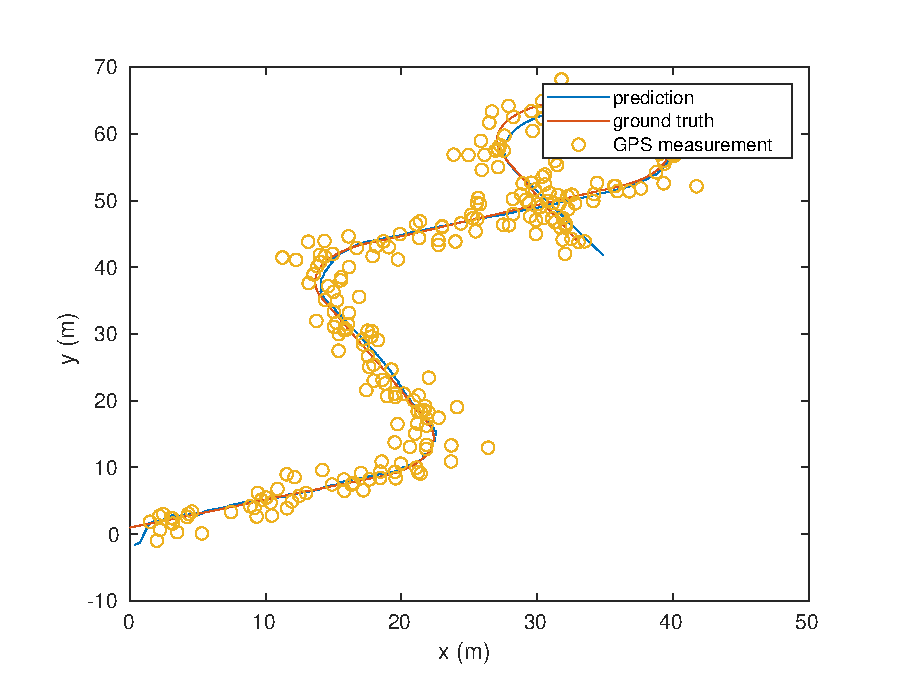
\includegraphics[width=\maxwidth{83.69292523833417em}]{figure_1.eps}
\end{center}
\begin{matlabcode}

plot(t_2, tau_m);
title('tau m vs time')
ylabel('tau m')
xlabel('time')
\end{matlabcode}
\begin{center}
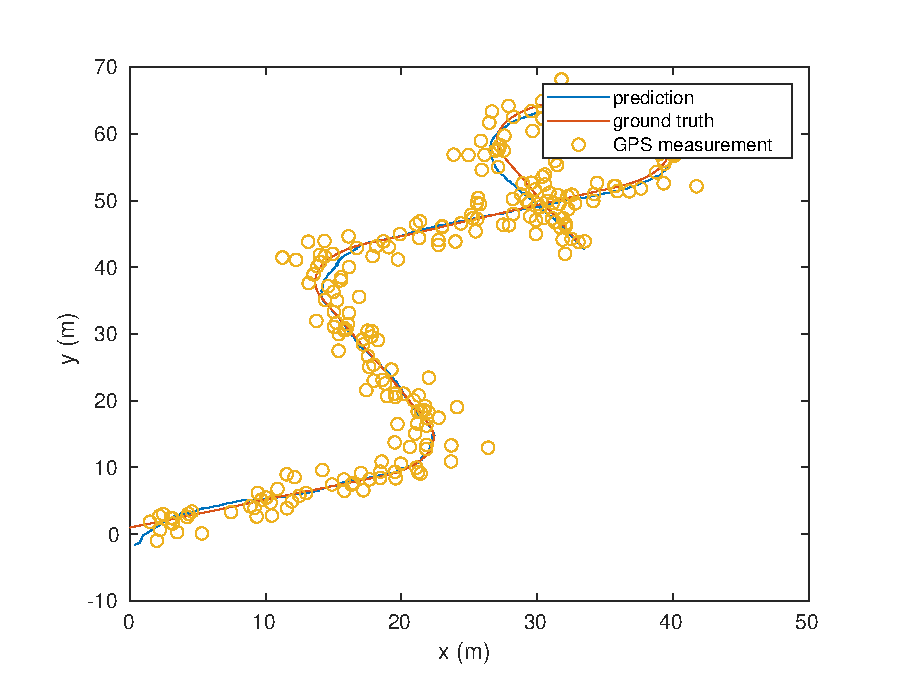
\includegraphics[width=\maxwidth{83.69292523833417em}]{figure_2.eps}
\end{center}
\begin{matlabcode}

\end{matlabcode}

\end{document}
